\section{Descrizione del progetto}
Per quanto riguarda il progetto realizzato in cpp si è pensato, piuttosto che realizzare un applicativo "funzionale" (approccio seguito per gli altri 3 progetti), di andare a realizzare una libreria per il calcolo numerico, che consiste in due moduli principali:
\begin{itemize}
	\item Matrici
	\item Applicativo dimostrativo
\end{itemize}

In particolare sono state sviluppate alcune funzionalità algebriche base come \textbf{somma} e \textbf{sottrazione} elemento per elemento di una matrice: l'espressività del C++ ha permesso di rendere questa libreria del tutto generica, permettendo quindi di realizzare matrici composte da elementi di qualsiasi tipo, tramite l'utilizzo dei \textbf{templates generici}.

\section{Gerarchia delle classi}
Come si vede nell'\textit{UML Class Diagram} in figura ~\ref{fig:UMLClassDiagram}, la libreria presenta una classe base principale, \textit{Number}, che rappresenta un numero il quale può essere un numero di tipo \textit{Addable} o \textit{Subtractable}, che offrono rispettivamente un metodo e un operatore per realizzare la somma e la sottrazione.
\begin{figure}[h]
	\centering
	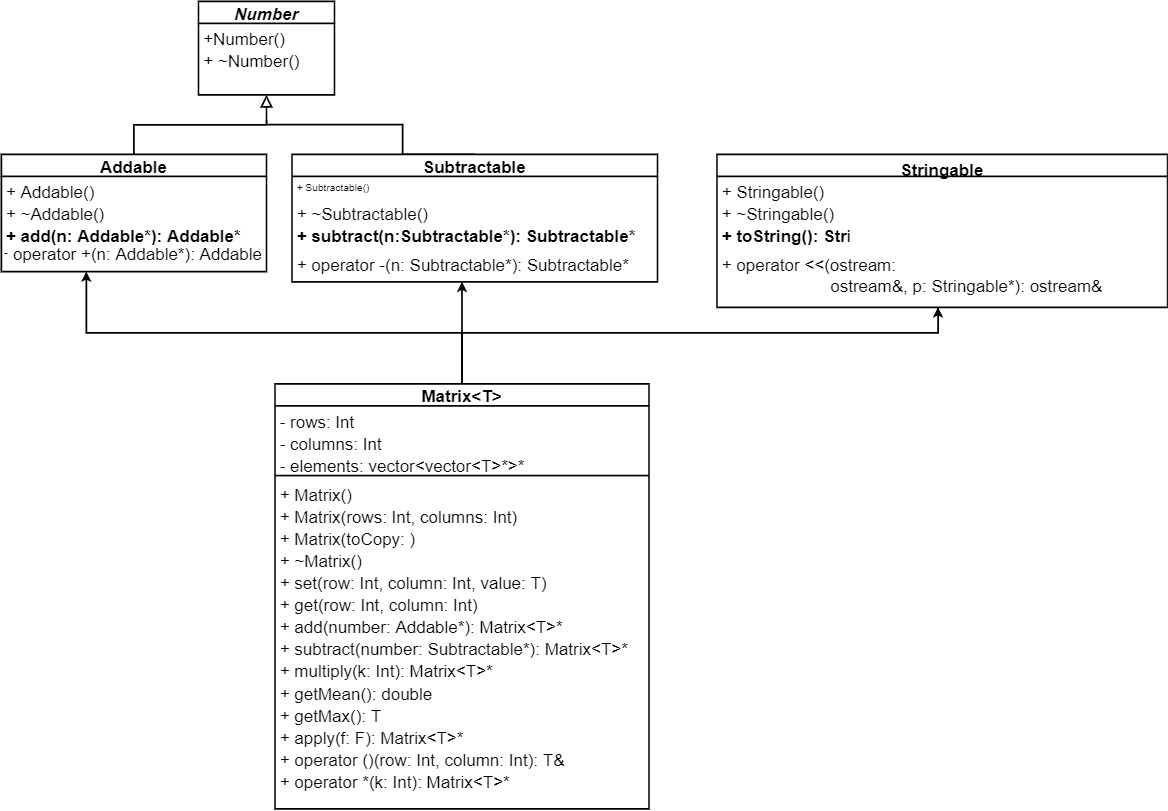
\includegraphics[width=0.7\textwidth]{Immagini/ClassDiagram.jpg}
	\caption{UML class diagram}
	\label{fig:UMLClassDiagram}
\end{figure}

\section{Multiple inheritance}
Nella gerarchia delle classi sopra esposta, è stato necessario utilizzare l’ereditarietà multipla
nei due diversi contesti tipici: 
\begin{itemize}
	\item \textbf{implementazione di interfacce}
	\item \textbf{ereditarietà multipla classica}
\end{itemize}

\textbf{Il C++ non fa distinzioni sostanziali tra queste due tipologie, ma la differenza concettuale è
notevole, tanto che altri linguaggi (come Java) i quali permettono di implementare più interfacce ma non di ereditare di più classi.}

La prima tipologia consiste nel derivare una classe da al più una classe base “non pure virtual”.
Le altre classi base devono essere l’equivalente delle interface Java, ovvero devono essere
classi astratte (\textit{Abstract Base Classes} - ABCs) in cui tutte le member functions sono
pure virtual.

\textbf{Questa tipologia di eredità è stata utilizzata per derivare da Stringable}.

La seconda tipologia di eredità è stata invece utilizzata per andare a modellizzare il rapporto tra una matrice e quelle che sono le strutture relative a \textbf{Number}, come si vede nella figura ~\ref{fig:MultipleInerithance}.

\begin{figure}[h]
	\centering
	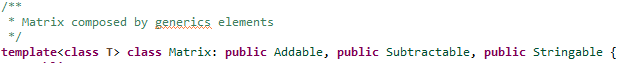
\includegraphics[width=0.6\textwidth]{Immagini/MultipleInerithance.png}
	\caption{Esempio di eredità multipla della classe \textit{Matrix}}
	\label{fig:MultipleInerithance}
\end{figure}

\section{Diamond inheritance}
Un aspetto problematico dell’ereditarietà multipla (specialmente quando si attua una doppia ereditarietà da due classi diverse, la quale è una peculiarità del C++) è la
possibilità di generare una \textbf{gerarchia a diamante}.

Essa si verifica quando, come si vede nella figura ~\ref{fig:DiamondProblem}, una generica classe D eredita da due classi B e C che hanno un antenato in comune A. In questo caso c'è un'ambiguità su quale “versione” dell'antenato deve essere ereditata da D: quella di B o quella di C?

\begin{figure}[h]
	\centering
	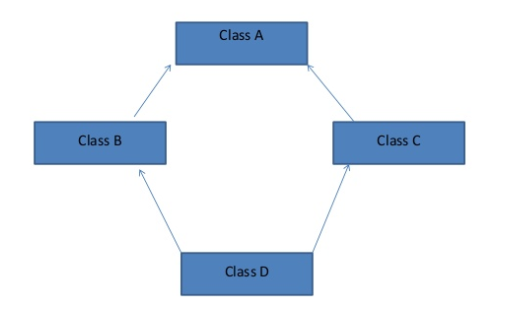
\includegraphics[width=0.3\textwidth]{Immagini/DiamondProblem.png}
	\caption{Diamond problem}
	\label{fig:DiamondProblem}
\end{figure}

Un modo di risolvere il problema in C++ è dichiarare, nelle classi B e C, un'\textbf{eredità virtuale} da A, specificandolo direttamente nella dichiarazione, come fatto nelle classi \textbf{Addble} e \textbf{Subtractable} (figura ~\ref{fig:VirtualInerithance}).

\begin{figure}[h]
	\centering
	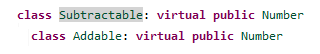
\includegraphics[width=0.5\textwidth]{Immagini/VirtualInerithance.png}
	\caption{Virtual Inerithance nelle classe \textit{Addable} e \textit{Subtractable}}
	\label{fig:VirtualInerithance}
\end{figure}

\section{Costruttori e distruttori}
\subsection{Costruttori}
La libertà di poter utilizzare oggetti all'interno delle applicazioni scritte in C++, si incontra però con la necessità di andare a compiere due operazioni preliminari:
\begin{itemize}
	\item Allocare la memoria dei membri dell'oggetto in esame;
	\item Inizializzate i membri.
\end{itemize}
Queste operazioni sono svolte da una particolare funzione membro detta \textbf{costruttore}, il cui nome coincide con quello della classe e non presenta alcun valore di ritorno.

In C++ un costruttore che non accetta argomenti, o in cui tutti gli argomenti sono opzionali, è detto \textbf{costruttore di default} ed è possibile sovraccaricare questo metodo, fornendo quindi diverse alternative. E' comunque sempre buona norma andare a realizzare l'overloading del costruttore di default, perchè esso ha dei limiti come il fatto che il valore predefinito per il tipo di ogni dato membro può dipendere dal compilatore utilizzato, e quindi non essere deterministico.

\subsection{Distruttori}
Dal lato opposto, il \textbf{distruttore} si occupa del compito di rilasciare tutte le risorse associate ad un oggetto, quando finisce la lifetime dell'oggetto stesso: infatti il distruttore viene invocato per tutte le variabili automaticamente ogni volta che viene raggiunta la fine del loro \textit{scope} e tutte le volte che le variabili dinamiche vengono deallocate con la parola chiave \textit{delete}.

In particolare, come per il costruttore, anche il distruttore presenta una firma particolare, ovvero presenta lo stesso nome della classe solamente per il fatto che è preceduto dal simbolo ~ (\textit{tilde}); anch'esso, come il costruttore, non presenta alcun valore di ritorno, e in più non presenta parametri (motivo per cui non può essere sovraccaricato).

Inoltre se non viene esplicitamente incluso nella dichiarazione della classe, il distruttore viene generato automaticamente dal compilatore. In questo caso tuttavia, l’unica risorsa rilasciata è la memoria occupata dall’oggetto: se alcuni dei suoi dati membro sono delle reference, o se l’oggetto fa uso di altre risorse (file o altre interfacce di I/O), potrebbe essere necessario svolgere delle operazioni per il loro corretto rilascio.

\subsection{Implementazione nell'applicazione}
Queste caratteristiche sono state sfruttate per quanto riguarda gli oggetti della classe \textit{Matrix}.

Per quanto riguarda la costruzione degli oggetti di tipo \textit{Matrix} sono stati sovraccaricati i costruttori di default, con 2 alternative differenti: come si vede in figura ~\ref{fig:matrixInit}

\begin{figure}[h]
	\centering
	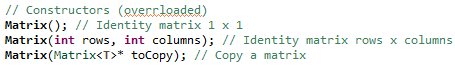
\includegraphics[width=0.8\textwidth]{Immagini/MatrixConstructors.png}
	\caption{Costruttori classe \textit{Matrix}}
	\label{fig:matrixInit}
\end{figure}

In particolare si ha che:
\begin{itemize}
	\item Il primo costruttore rappresenta il costruttore di default, ed è stato implementato per fornire un'inizializzazione "custum" (e non di default del compilatore) ai membri della classe. Esso va a creare una matrice identità di dimensioni 1x1;
	\item Il secondo costruttore invece va a inizializzare i mebri della classe \textit{Matrix} in maniera tale da ricreare una matrice di dimensioni \textit{rows x columns} (parametri passati in input al costruttore);
	\item L'ultimo overriding del costruttore di \textit{Matrix} permette di inizializzare un nuovo oggetto \textit{Matrix} tramite un altro oggeto di tipo \textit{Matrix}.
\end{itemize}

Per quanto riguarda il distruttore (figura ~\ref{fig:matrixDeInit}) sono due gli aspetti da porre ini evidenza:
\begin{itemize}
	\item é stato definito \textit{virtual} in maniera tale che venissero chiamati anche i distruttori delle superclassi;
	\item esso si occupa, come si vede nella relativa implementazione, di andare a liberare la memoria allocata per la struttura contenete gli elementi della matrice: per fare ciò s è fatto uso di un iteratore sulle righe della matrice, in maniera tale da andare poi a liberare ogni elemento della colonna.
\end{itemize}

\begin{figure}[h]
	\centering
	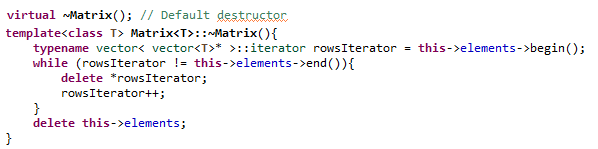
\includegraphics[width=0.8\textwidth]{Immagini/MatrixDestructors.png}
	\caption{Firma e implementazione del distruttore della classe \textit{Matrix}}
	\label{fig:matrixDeInit}
\end{figure}

\section{Overloading particolari}
Nella nostra libreria, su consigli di altri studenti, siamo andati a ridefinire alcuni operatori, per renderli più "personalizzati".
\subsection{Overloading di cout<<}
Tra gli operatori che risulta utili sovraccaricare c'è "<<", il quale è utilizzato nella libreria standard per inviare dati agli oggetti \textit{ostream} (flussi in output): è stato quindi possibile personalizzare, in maniera facile e diffusa, la tipologia di log aggiungendo, come si vede in figura ~\ref{fig:CoutRedef}, un print personalizzato, per distinguere così il log della libreria da quello di sistema classico.

\begin{figure}[h]
	\centering
	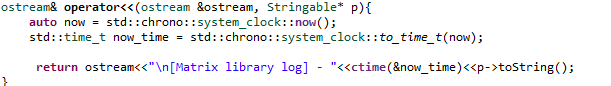
\includegraphics[width=0.8\textwidth]{Immagini/CoutRedefinition.png}
	\caption{Ridefinizione dell'operatore di stream}
	\label{fig:CoutRedef}
\end{figure}

\subsection{Overloading di ()}
L'operatore () è leggeremente diverso dagli altri, in quanto è possibile interpretarlo in due modi, a seconda che compaiano in un l-value ("get") o in un r-value ("set").

In C++ è possibile sovraccaricare gli operatori in modo che si comportino in maniera diversa a seconda della posizione esattamente come accade con gli array.

\begin{figure}[h]
	\centering
	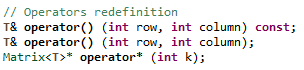
\includegraphics[width=0.5\textwidth]{Immagini/MatrixOperatorsRedef.png}
	\caption{Ridefinizione degli operatori nella classe \textit{Matrix}}
	\label{fig:MatrixOperatorRedef}
\end{figure}

Nella nostra applicazione siamo andati a ridefinire appunto l'operatore (), come si vede in figura ~\ref{fig:MatrixOperatorRedef}, in particolare:
\begin{itemize}
	\item  la presenza del simbolo \textbf{$\&$} subito dopo il valore ritornato indica che ci sono\textbf{ due definizioni diverse dello stesso operatore}.
	\item il modificatore \textbf{const} indica invece che la\textbf{ prima ridefinizione è quella da usare se l'operatore sta a sinistra} (\textit{l-value}) del simbolo di assegnamento.
\end{itemize}
Un esempio di applicazione della redefinizione dell'operatore (), li si possono vedere in figura ~\ref{fig:OperatorExamples}.

\begin{figure}[h]
	\centering
	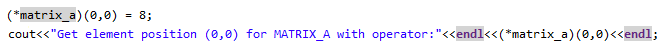
\includegraphics[width=0.8\textwidth]{Immagini/OperatorExample.png}
	\caption{Esempio di utilizzo della redefinizione degli operatori}
	\label{fig:OperatorExamples}
\end{figure}

\section{Templates}
Un metodo più potente per il riutilizzo del codice è fornito dai templates. 

Essi costituiscono uno “schema” di classe che poi verrà realizzato concretamente sostituendo ai tipi parametrici i tipi effettivi dichiarati dagli utilizzatori.

A differenza del linguaggio Java, ogni differente realizzazione del template costituisce un tipo
a sé stante e senza alcuna relazione con gli altri: in Java si può avere una gerarchia di tipi
derivati dallo stesso template.

In C++ invece ogni realizzazione di un template viene concretizzata tramite codice
indipendente, portando quindi ad un file eseguibile di dimensioni maggiori. Inoltre, per fornire
vincoli in modo esplicito come in Java, si deve ricorrere a una “pseudo-ereditarietà”.

Questa flessibilità offerta dai templates, è stata utilizzata nella stesura della classe \textit{Matrix}.

\section{Standard Template Library}
La libreria STL del C++ mette a disposizione una serie di contenitori parametrici, che quindi
possono contenere oggetti di tipo arbitrario. Fornisce inoltre iteratori che permettono di visitare
tali contenitori e algoritmi per manipolarne gli elementi.

Uno dei contenitori più semplici è \textit{vector}, una classe che permette di gestire collezioni di oggetti ordinati come un array.

I vantaggi del vector sul semplice array sono diversi, tra cui la gestione automatica della
memoria e la presenza di diversi metodi per le operazioni più comuni quali l'inserimento di un
nuovo valore.

La classe Matrix utilizza un vector per memorizzare gli elementi della matrice ed essendo
parametrica di parametro T, utilizza un \textit{vector<vector<T>>}.
\subsection{STL - Iterator}
Tra le altre funzionalità messe a disposizione da vector e dagli altri contenitori in STL ci sono gli
iteratori, che costituiscono il modo standard di accedere agli elementi nel contenitore stesso. Gli
iteratori si comportano in modo simile a semplici puntatori (ad esempio ammettono l'operatore ++),
anche se in realtà sono più flessibili e possono essere utilizzati anche con le liste.

\begin{figure}[h]
	\centering
	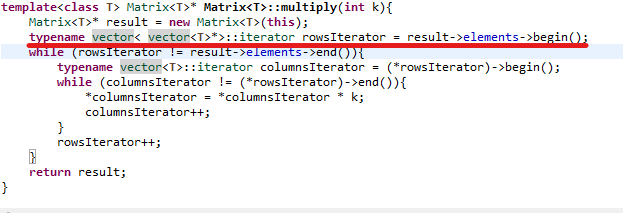
\includegraphics[width=0.7\textwidth]{Immagini/Stl_Iterator.png}
	\caption{STL - Iterator}
	\label{fig:Iterator}
\end{figure}

\subsection{STL - Algorithm}
La libreria STL mette a disposizione anche degli algoritmi generici e riutilizzabili per operare sui contenitori.

Tali algoritmi sono implementati tramite funzioni template che si possono includere nei propri file tramite la direttiva di include.

Un esempio di algoritmo è la funzione \textit{for-each()}, che applica una funzione parametro a tutti gli
elementi di un contenitore.

\begin{figure}[h]
	\centering
	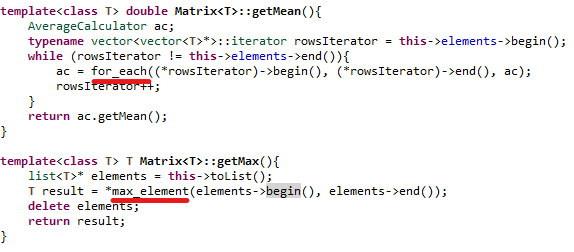
\includegraphics[width=0.7\textwidth]{Immagini/Stl_Algorithm.png}
	\caption{STL - Algorithm}
	\label{fig:Algoritm}
\end{figure}